\subsection{Clustering Losses}

\begin{frame}
	\frametitle{Clustering Losses}
	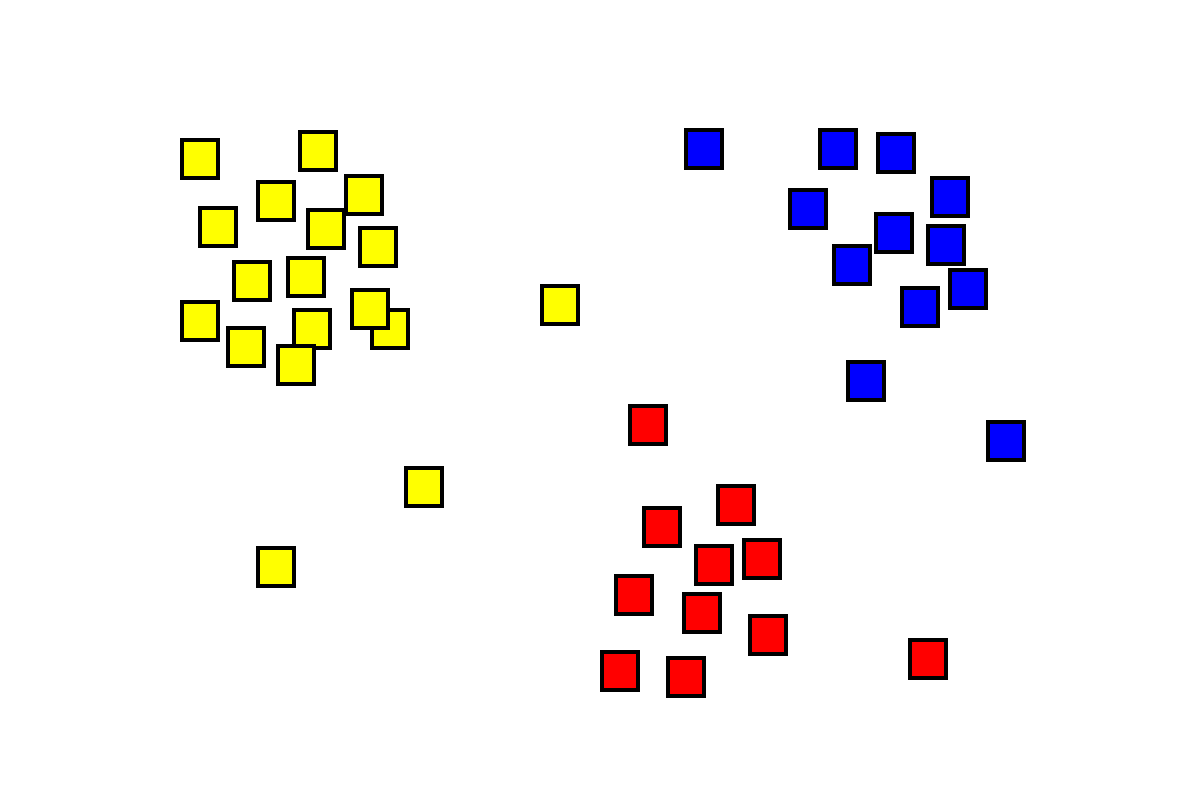
\includegraphics[scale=0.2, center]{images/clust1}
\end{frame}

\begin{frame}
	\frametitle{Mean Entropy Loss}
	\begin{itemize}
		\item The mean entropy loss over a batch of size $T$ is gives by:
			\begin{block}{MEL}
				\begin{equation*}
					J_M = \frac{1}{T}\sum_{t=1}^{T}H(\mathbf{q}_t)
				\end{equation*}
				where $H$ is the entropy and $\mathbf{q}_t = f(\mathbf{X}_t; \Theta)$ is the output
				probability distribution for image $\mathbf{X}_t$
			\end{block}
			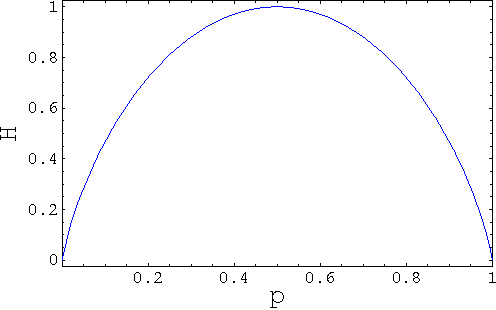
\includegraphics[scale=0.18, center]{images/ent.png}
		\item This increases the confidence of the predicted class
	\end{itemize}
\end{frame}

\begin{frame}
	\frametitle{Negative Batch Entropy Loss}
	\begin{itemize}
		\item The spread of outputs should be similar to the dataset
			label distribution
			\begin{block}{NBEL for Uniform Dataset Label Distribution}
				\begin{equation*}
					J_B = -H(\bar{\mathbf{q}})
				\end{equation*}
				where,
				\begin{equation*}
					\bar{\mathbf{q}} = \frac{1}{T}\sum_{t=1}^{T}\mathbf{q}_t
				\end{equation*}
			\end{block}

	\end{itemize}
\end{frame}

\begin{frame}
	\frametitle{Negative Batch Entropy Loss}
	\begin{itemize}
		\item Can be generalized to any distribution
			\begin{block}{Negative Batch Entropy Loss}
				\begin{equation*}
					\label{eq:nbel}
					J_B = D_{KL} (\bar{\mathbf{q}} \lVert \mathbf{d})
				\end{equation*}
				where $D_{KL}$ is the KL-divergence, and $\mathbf{d}$ is
				the empirical class distribution estimated from $\mathcal{S}$
			\end{block}

	\end{itemize}
\end{frame}

